\documentclass{beamer}

\usepackage{graphicx}
\usepackage{textpos}

\usetheme{Madrid}
\useoutertheme{miniframes} % Alternatively: miniframes, infolines, split

% Setup the university's color pallette
\definecolor{UIUCorange}{RGB}{19, 41, 75} % UBC Blue (primary)
\definecolor{UIUCblue}{RGB}{232, 74, 39} % UBC Grey (secondary)


\setbeamercolor{palette primary}{bg=UIUCorange,fg=white}
\setbeamercolor{palette secondary}{bg=UIUCblue,fg=white}
\setbeamercolor{palette tertiary}{bg=UIUCblue,fg=white}
\setbeamercolor{palette quaternary}{bg=UIUCblue,fg=white}
\setbeamercolor{structure}{fg=UIUCorange} % itemize, enumerate, etc
\setbeamercolor{section in toc}{fg=UIUCblue} % TOC sections

\setbeamercolor{subsection in head/foot}{bg=UIUCorange,fg=UIUCblue}
\setbeamercolor{subsection in head/foot}{bg=UIUCorange,fg=UIUCblue}

\usepackage[utf8]{inputenc}
\usepackage{graphicx}


%Information to be included in the title page:
\title{\textbf{Introduction to the Course}}
\author{\textbf{David H Smith IV}}
\institute[\textbf{UIUC}]{\textbf{University of Illinois Urbana-Champaign}}
\date{\textbf{Mon, June 14 2021}}

\setbeamertemplate{title page}[default][colsep=-4bp,rounded=true]
\addtobeamertemplate{title page}{\vspace{3\baselineskip}}{}
\addtobeamertemplate{title page}{
  \begin{textblock*}{\paperwidth}(-1.0em, -1.2em)
    
\includegraphics[width=\paperwidth, height=\paperheight]{imgs/uiuc.png}
  \end{textblock*} 
}{}

\begin{document}

\frame{\titlepage}


%
% Slide 1
%
\begin{frame}
  \frametitle{Course Outcomes}
  \begin{itemize}
    \item Given a small section of code you should be able to:
      \begin{itemize}
        \item Trace through and predict it's output.
        \item Describe, in plain English, what it does.
      \end{itemize}
    \item Write a small python program some, or all, of the fundamentals you will learn in the course.
    \item Beginner and intermediate spreadsheet operations.
    \item Beginner level understanding of how the internet works and how to write basic HTML documents.
  \end{itemize}
\end{frame}
%
% Slide 2
%
\begin{frame}
  \frametitle{What is Computer Science?}
  \begin{itemize}
    \item CS is concerned with understanding:
      \begin{itemize}
        \pause
        \item What is computable
        \pause
        \item How to compute it in one or more of the following in mind:
          \begin{itemize}
            \pause
            \item Speed
            \pause
            \item Reliability
            \pause
            \item Security 
            \pause
            \item Resource cost
          \end{itemize}
        \pause
      \end{itemize}
  \end{itemize}
\end{frame}


%
% Slide 3
%
\begin{frame}
  \frametitle{What is Programming?}
  \begin{minipage}{0.5\textwidth}
    \begin{itemize}
      \item Programming $\neq$ Computer Science
        \begin{itemize}
          \item Rather, programming is a subset of Computer Science
        \end{itemize}
      \pause
      \item ``Computer Science is no more about computers than astronomy is about telescopes'' - Edsger W. Dijkstra
        \begin{itemize}
          \item A bit of an overstatement but still a useful thing to keep in mind.
        \end{itemize}
      \pause
      \item \textbf{High Level Definition: } A series of instructions that a computer carries out.
    \end{itemize}
  \end{minipage}
  \begin{minipage}{0.5\textwidth}
  \end{minipage}
\end{frame}

%
% Slide 4
%
\begin{frame}
  \frametitle{Where did this all come from?}
\end{frame}

%
% Slide 5
%
\begin{frame}
  \frametitle{Early ``Computers''}
\end{frame}

%
% Slide 6
%
\begin{frame}
  \frametitle{The Difference Engine}
\end{frame}

%
% Slide 7
%
\begin{frame}
  \frametitle{Alan Turing, Alonzo Church, and Turing Machines}
  \begin{minipage}{0.59\textwidth}
    \begin{enumerate}
      \item \textbf{Church-Turing thesis} - Any effective calculation can be performed by a mechanical computer (e.g., a Turing Machine).
      \item \textbf{Turing Machines} - An abstract, mathematical model of a machine that moves up and down a strip of paper, one step at a time, and performs operations based on a set of rules (Figure 1).
    \end{enumerate}
  \end{minipage}
  \begin{minipage}{0.39\textwidth}
    \begin{figure}
      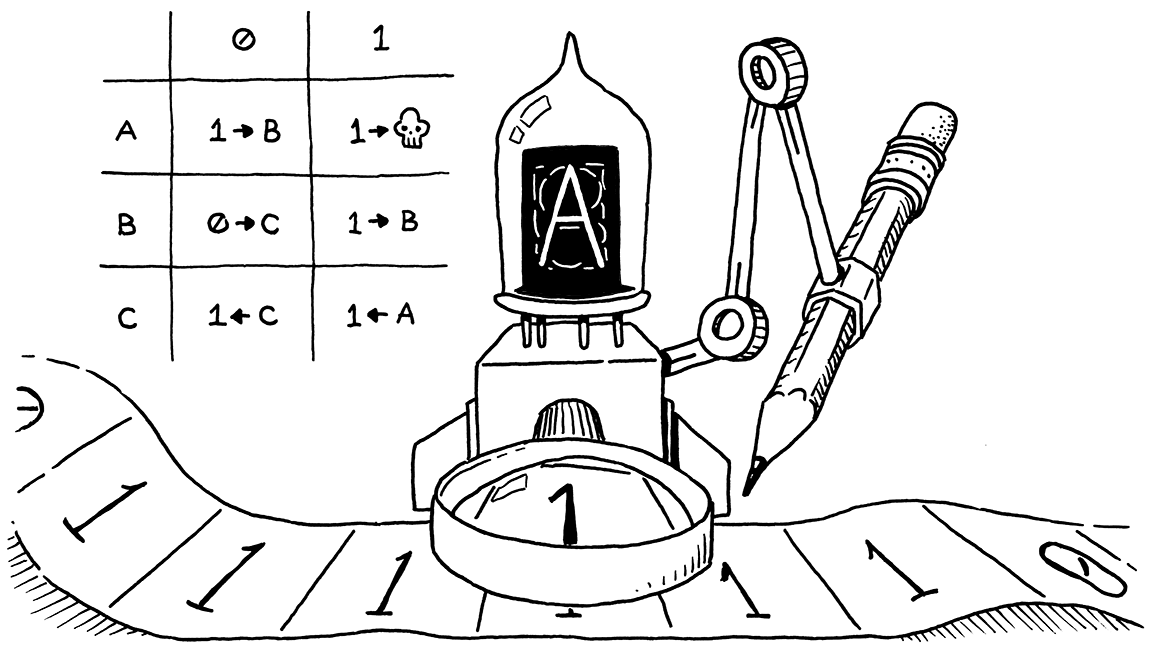
\includegraphics[width=\textwidth]{imgs/turing-machine.png}
    \end{figure}
  \end{minipage}
\end{frame}

%
% Slide 8
%
\begin{frame}
  \frametitle{}
\end{frame}

%
% Slide 4
%
\begin{frame}
  \frametitle{}
\end{frame}

%
% Slide 4
%
\begin{frame}
  \frametitle{}
\end{frame}




\end{document}
